\chapter{Introduction}

\dictum[Теодо́сій Григо́рович Добжа́нський (Theodosius
Dobzhansky)\footnotemark]{Nothing in biology makes sense}
\footnotetext{\citet{Dobzhansky:1973}}

\section{The central dogma}

At the core of every living being is its genetic inheritance. The genetic
inheritance is what is being passed down from parents to their offspring, and
contains a blueprint detailing how to construct a new individual in a process
called \define{embryogenesis}. This genetic inheritance is physically present in
the form of \dna in every living cell.\footnote{And to some extent in non-living
particles called \define{viruses}.}

If the \dna is a library containing a blueprint of the cell’s instructions, then
there is need also for librarians, and for workers who enact the instructions
found in the blueprint and conveyed by the librarians. These find their
counterparts in living cells in the form of \mrna and \define{proteins}. The
process by which genetic information is stored in the \dna, conveyed by
\mrna[s], and enacted by proteins is formalised in the \emph{central dogma of
molecular biology}.

\begin{figure}[h!]
    \centering
    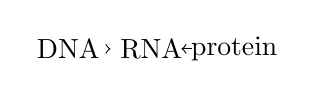
\begin{tikzpicture}
        [every node={circle, draw, inner sep=1em}, node distance=3em]
        \node (dna) {DNA};
        \node (rna) [right of=dna] {RNA};
        \node (protein) [right of=rna] {protein};
        \draw [->] (dna) -- (rna);
        \draw [->] (rna) -- (protein);
    \end{tikzpicture}
    \figcap{dogma}{The central dogma of molecular biology.}{}
\end{figure}

This very high-level view needs to be complemented by a more mechanistic
description in order to make sense. All three roles in the central dogma are
fulfilled by different molecules. \dna consists of a long chain of
\define{nucleotides}. The chemical nature of nucleotides means that these will
easily polymerase into long, relatively stable chains. \dna is made up of four
different types of nucleotides: adenine (\nA), cytosine (\nC), guanine (\nG) and
thymine (\nT). Thus, \dna can be thought of as a long string of four letters,
and that is indeed how it is often represented. Text is read from left to right
in Western culture. \dna is read from \fivep to \threep.\footnote{Referring to
the number of the phosphate atom in each nucleotide, which is exposed at either
end of the chain.}

\dna is present in the cell in the form of double-stranded helices: each \dna
molecule consists of two paired chains, wound rightly around each other, with
the bases on each chain pairing up such that every \nA on one chain is paired
with a \nT on the other, and each \nC is paired with a \nG. This striking
symmetry is known as Watson–Crick base pairing, after its discoverers
\citep{Watson:1953}. Thus, \dna is made up of two complementary strands,
redundantly holding the genetic information. This redundancy is used in \dna
copying (which occurs at every cell division, and is the mechanism by which
genetic information is passed from one cell to its offspring) to synthesise two
newly formed \dna molecules, of which each contains one strand of the parent
\dna molecule (\define{semiconservative replication}).

\todo[inline]{\begin{enumerate}[noitemsep,nolistsep,leftmargin=*]
    \item Molecular structure of DNA (bases, 5'--3', phosphoribose)
    \item DNA copying (strands, complementarity)
    \item Central dogma
    \item Template, coding strand, mRNA, proteins, genetic code
    \item Different polymerases, ncRNA
    \item DNA sequence as string
    \item Molecular and functional structure description of pol2 and pol3
\end{enumerate}}

\todo{Take intro from paper}

\subsection{Aside: modern modifications to the central dogma and evolution}

\subsection{Transcription}

\subsection{Posttranscriptional modification}

In particular A-to-I conversion (deamination), which is relevant in tRNA gene
wobble base pairing!

\subsection{Translation}

\subsection{The role of \abbr{trna}s in translation}

\section{Gene expression and its regulation}

\section{Using high-throughput sequencing for whole-genome analysis}

\subsection{Explain history and technology of \abbr{hts}}

\section{Types of non-coding \abbr{rna}, their function and expression}

\section{Structure of this thesis}
